\documentclass{article}
\usepackage{makeidx}
\usepackage{hyperref}
\usepackage{amsmath}
\usepackage{amssymb}
\usepackage{xcolor}
\usepackage{graphicx}

\title{Deep Learning Notes}
\author{Haotian Chen}
\date{}

\makeatletter
\renewcommand\paragraph{\@startsection{paragraph}{4}{\z@}%
                                     {-3.25ex\@plus -1ex \@minus -.2ex}%
                                     {1.5ex \@plus .2ex}%
                                     {\normalfont\normalsize\bfseries}}
\makeatletter

\hypersetup{
    colorlinks=true,
    linkcolor=blue,
    urlcolor=cyan,
}

\setcounter{tocdepth}{4}
\setcounter{secnumdepth}{4}

\makeindex



\begin{document}

\maketitle

\clearpage

\tableofcontents{}

\clearpage

\section{Neural Networks and Deep Learning}

\subsection{Activation Function}

\noindent \textbf{binary step:}

\begin{center}
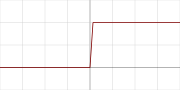
\includegraphics[scale=0.8]{./images/binary_step.png}
\end{center}

\[f(x) = \begin{cases}0&{\text{if }}x<0\\1&{\text{if }}x\geq 0\end{cases}, f(x) \in \{0, 1\}\]
\[f'(x) = \begin{cases}0&{\text{if }}x\neq 0\\{\text{undefined}}&{\text{if }}x=0\end{cases}\]

\noindent \textbf{sigmoid function:} (mainly used in output layer)

\begin{center}
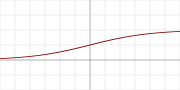
\includegraphics[scale=0.8]{./images/sigmoid.png}
\end{center}

\[f(x) = \sigma (x)={\frac {e^{x}}{e^{x}+1}}={\frac {1}{1+e^{-x}}}, f(x) \in (0, 1)\]
\[f'(x) = f(x)(1-f(x))\]

\noindent \textbf{rectified linear unit:}  (relu, mainly used in hidden layer)

\begin{center}
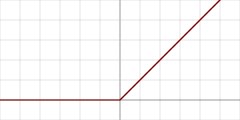
\includegraphics[scale=0.6]{./images/relu.png}
\end{center}

\[f(x) = max\{0, x\} = \begin{cases}0&{\text{if }}x<0\\1&{\text{if }}x\geq 0\end{cases}, f(x) \in [0, +\infty)\]
\[f'(x) = \begin{cases}0&{\text{if }}x<0\\1&{\text{if }}x>0\\{\text{undefined}}&{\text{if }}x=0\end{cases}\]

\noindent \textbf{Leaky rectified linear unit:}  (leaky relu, mainly used in hidden layer)

\begin{center}
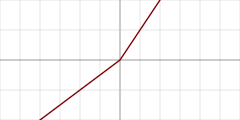
\includegraphics[scale=0.6]{./images/leaky_relu.png}
\end{center}

\[f(x) = \begin{cases}0.01x&{\text{if }}x<0\\x&{\text{if }}x\geq 0\end{cases}, f(x) \in (- \infty, + \infty)\]
\[f'(x) = \begin{cases}0.01&{\text{if }}x<0\\1&{\text{if }}x\geq 0\end{cases}\]

\noindent \textbf{hyperbolic tangent:} (tanh, mainly used in hidden layer)

\begin{center}
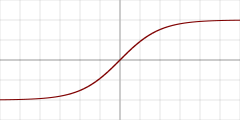
\includegraphics[scale=0.6]{./images/tanh.png}
\end{center}

\[f(x) = \tanh(x) = \frac {e^{x}-e^{-x}}{e^{x}+e^{-x}}, f(x) \in (-1, 1)\]
\[f'(x) = 1-f(x)^{2}\]

\noindent It turns out that the tanh activation usually works better than sigmoid activation function for hidden units because the mean of its output is closer to zero, and so it centers the data better for the next layer. Sigmoid or Tanh function disadvantage is that if the input is too small or too high, the slope will be near zero which will cause us the vanishing gradient problem.

\bigskip

\noindent Linear activation function will output linear activations. No matter how many hidden layers you add, the activation will be always linear like logistic regression (So its useless in a lot of complex problems). You might use linear activation function in the output layer if the output is real numbers (regression problem).

\subsection{Computation Graphs of Derivatives:}

\begin{center}
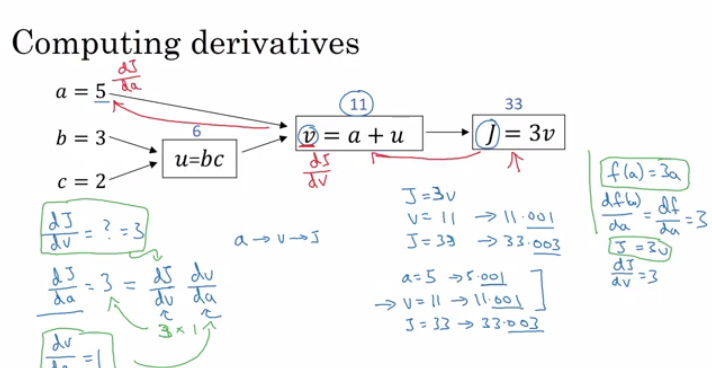
\includegraphics[scale=0.6]{./images/computation_graph.png}
\end{center}

\noindent apply chain rule:

\[\frac{\partial J}{\partial a} = \frac{\partial J}{\partial v} \frac{\partial v}{\partial a} = 3 \times 1 = 3\]

\[\frac{\partial J}{\partial b} = \frac{\partial J}{\partial v} \frac{\partial v}{\partial u} \frac{\partial u}{\partial b} = 3 \times 1 \times 2 = 6\]

\[\frac{\partial J}{\partial c} = \frac{\partial J}{\partial v} \frac{\partial v}{\partial u} \frac{\partial u}{\partial c} = 3 \times 1 \times 3 = 9\]


\subsection{Binary Classification}

Use logistic regression to build a binary classifier.

\begin{center}
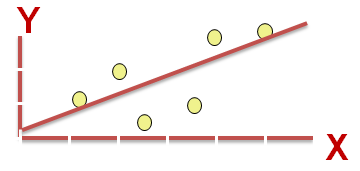
\includegraphics[scale=0.4]{./images/binary_classification.png}
\end{center}

\noindent \textbf{training data:}
\[x \in \mathbb{R}^{n_x}, y \in \{0, 1\}\]
\[\text{\(m\) training examples: } (x^{(i)}, y^{(i)})\:for\:i = 1, \dots, m\]

\[
x^{(i)} = 
\begin{bmatrix}
x^{(i)}_1\\
x^{(i)}_2\\
\vdots\\
x^{(i)}_n
\end{bmatrix}
,
y^{(i)} = y^{(i)}_1
\]

\[X =
\begin{bmatrix}
x^{(1)} & x^{(2)} & \dots & x^{(m)}
\end{bmatrix}
,
Y =
\begin{bmatrix}
y^{(1)} & y^{(2)} & \dots & y^{(m)}
\end{bmatrix}
\]

\[X \in \mathbb{R}^{n_x \times m}, Y \in \mathbb{R}^{1 \times m}\]

\subsection{Logistic Regression}

\noindent Logistic regression is a statistical model that uses a logistic function to model a binary dependent variable.

\bigskip

\noindent Given \(x\), want \(\hat{y} = P(y = 1 | x)\), where \(0 \leq \hat{y} \leq 1\), \(x \in \mathbb{R}^{n_x}\), \(w \in \mathbb{R}^{n_x}\), \(b \in \mathbb{R}\)

\[z = w^Tx + b\]
\[\hat{y} = \sigma(z) = \frac {1}{1+e^{-z}}\]

\[P(y|x) = \begin{cases}\hat{y}&{\text{if }}y = 1\\1 -\hat{y}&{\text{if }}y = 0\end{cases} = \hat{y}^y (1 - \hat{y})^{(1 - y)}\]

\noindent We want to maximize \(P(y|x)\). To make it simpler, because \(log\) function is a strictly increasing function, we can maximize \(log(P(y|x))\) instead.

\[log(P(y|x)) = log(\hat{y}^y (1 - \hat{y})^{(1 - y)}) = ylog(\hat{y}) + (1 - y)log(1 - \hat{y})\]

\noindent Or in reverse, we can minimize \(-log(P(y|x))\), which is called \textbf{loss function}.

\noindent \textbf{loss function: (convex)}

\[L(\hat{y}, y) = -(ylog(\hat{y}) + (1 - y)log(1 - \hat{y}))\]

\noindent \textbf{cost function: (convex)}

\[J(w, b) = \frac{1}{m} \sum^m_{i = 1} L(\hat{y}^{(i)}, y^{(i)}) = - \frac{1}{m} \sum^m_{i = 1} [y^{(i)}log(\hat{y}^{(i)}) + (1 - y^{(i)})log(1 - \hat{y}^{(i)})]\]

\noindent \textbf{gradient descent:} with learning rate \(\alpha\), find best \(w\), \(b\) to minimize \(J(w, b)\)

\noindent repeat until convergence \{
\[w_j =: w_j - \alpha \frac{\partial}{\partial w_j} J(w, b) = w_j - \alpha \frac{1}{m} \sum^m_{i = 1} (\hat{y}^{(i)} - y^{(i)}) x^{(i)}_j\]
\[b =: b - \alpha \frac{\partial}{\partial b} J(w, b) = b - \alpha \frac{1}{m} \sum^m_{i = 1} (\hat{y}^{(i)} - y^{(i)})\]
\centerline{simultaneously update \(w_j\) and \(b\), \(j \in [1, n]\)}
\}

\bigskip

\noindent \textbf{vectorized implementation}:

\noindent repeat until convergence \{
\[w =: w - \alpha \frac{1}{m} X (\sigma(w^TX + b) - Y)^T\]
\[b =: b - \alpha \frac{1}{m} sum\{\sigma(w^TX + b) - Y\}\]
\}

\subsection{Neural Network}

\noindent \textbf{Basic Structure:}

\begin{center}
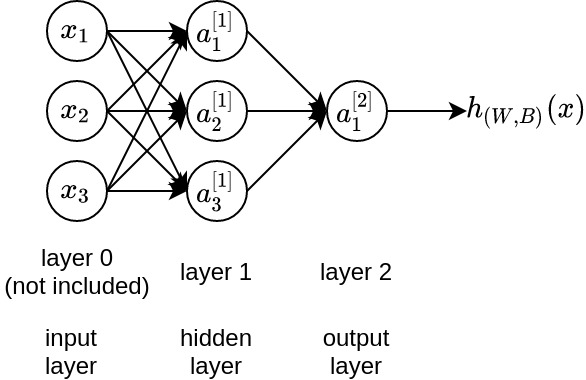
\includegraphics[scale=0.4]{./images/neural_network.jpg}
\end{center}
\[a_i^{[j]} = \text{"activation" of unit i in layer j}\]
\[W^{[j]} = \text{matrix of weights (edges) from layer j - 1 to j}\]
\[B^{[j]} = \text{vector of biases (nodes) from layer j - 1 to j}\]

\[a_1^{[1]} = \sigma(W_{11}^{[1]} x_1 + W_{12}^{[1]} x_2 + W_{13}^{[1]} x_3 + B_{1}^{[1]})\]
\[a_2^{[1]} = \sigma(W_{21}^{[1]} x_1 + W_{22}^{[1]} x_2 + W_{23}^{[1]} x_3 + B_{2}^{[1]})\]
\[a_3^{[1]} = \sigma(W_{31}^{[1]} x_1 + W_{32}^{[1]} x_2 + W_{33}^{[1]} x_3 + B_{3}^{[1]})\]
\[h_{(W, B)}(x) = a_1^{[2]} = \sigma(W_{11}^{[2]} a_1^{[1]} + W_{12}^{[2]} a_2^{[1]} + W_{13}^{[2]} a_3^{[1]} + B_{1}^{[2]})\]

\bigskip

\noindent If network has \(s_j\) units in layer \(j\), \(s_{j - 1}\) units in layer \(j - 1\), then \(W^{[j]}\) will be of dimension \(s_j \times s_{j - 1}\), \(B^{[j]}\) will be of dimension \(s_j \times 1\).

\bigskip

\noindent \textbf{Generalized Model (one vs all):}

\begin{center}
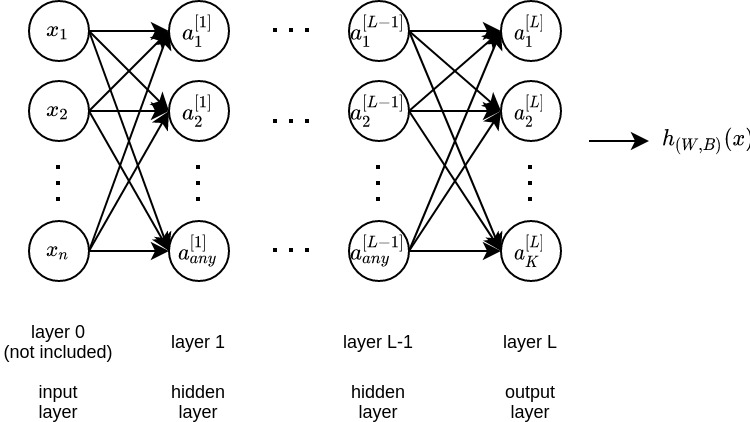
\includegraphics[scale=0.4]{./images/neural_network_generalized.jpg}
\end{center}

\noindent For a neural network that has:

\[L = \text{total number of layers in the network}\]
\[s_l = \text{number of units in layer } l\]
\[K = \text{number of output units/classes}\]

\noindent assume \(a^{[0]} = x, a^{[L]} = h_{(W, B)}(x)\), let:

\[z^{[l]} = W^{[l]} a^{[l - 1]} + B^{[l]}\]
\[a^{[l]} = \sigma(z^{[l]})\]
\[h_{(W, B)}(x) = a^{[L]} = \sigma(z^{[L]})\]

\bigskip

\noindent \textbf{regularized cost function:}
\[J(W, B) = - \frac{1}{m} \sum_{i = 1}^{m} \sum_{k = 1}^{K} [y^{(i)}_k log(h_{(W, B)} (x^{(i)})_k) + (1 - y^{(i)}_k) log(1 - h_{(W, B)}(x^{(i)})_k)] + \frac{\lambda}{2m} \sum_{l = 1}^{L} \sum_{i = 1}^{s_l} \sum_{j = 1}^{s_{l + 1}} (W_{j, i}^{[l]})^{2}\]

\noindent To reduce over-fitting, we can reduce(penalize) the weight of the features in our function carry by increasing their cost. The \(\lambda\) is the regularization parameter. It determines how much the costs of our theta parameters are inflated.

\bigskip

\noindent \textbf{vectorized implementation}: (with different activation function for each layer)

\[Z^{[l]} = W^{[l]}A^{[l - 1]} + B^{[l]}\]
\[A^{[l]} = \sigma^{[l]}(Z^{[l]})\]
\[h_{(W, B)}(X) = A^{[L]} = \sigma^{[L]}(Z^{[L]})\]
\[J(W, B) =  - \frac{1}{m} np.sum(Y \odot log(h_{(W, B)}(X)) + (1 - Y) \odot log(1 - h_{(W, B)}(X))) + \frac{\lambda}{2m} np.sum(W \odot W)\]

\subsection{Backpropagation Preliminary}
\noindent \textbf{matrix calculus:} see \href{https://en.wikipedia.org/wiki/Matrix_calculus}{Wikipedia}

\noindent \textbf{chaine rule:}

\noindent Suppose the variable \(J\) depends on the variables \(w_1, \dots, w_p\) via the intermediate variable \(z_1, \dots, z_k\).

\[z_j = z_j(w_1, \dots, w_p), \forall j \in \{1, \dots, k\} \]
\[J = J(z_1, \dots, z_k)\]

\noindent Expand \(J\), we can find:

\[\frac{\partial J}{\partial w_i} = \sum_{j = 1}^{k} \frac{\partial J}{\partial z_j} \frac{\partial z_j}{\partial w_i}, \forall i \in \{1, \dots, p\}\]

\noindent \textbf{chain rule derivation for matrix:}

\noindent Suppose \(J\) is a real-valued output variable, \(z \in \mathbb{R}^m\) is the intermediate variable and \(W \in \mathbb{R}^{m \times d}\), \(B \in \mathbb{R}^{m}\), \(a \in \mathbb{R}^d\) are the input variables. Suppose they satisfy:

\[z = W a + B\]
\[J = J(z)\]

\noindent Then we can get:

\[
\frac{\partial J}{\partial a} = 
\begin{bmatrix}
\frac{\partial J}{\partial a_1}\\
\vdots\\
\frac{\partial J}{\partial a_d}
\end{bmatrix}
= 
\begin{bmatrix}
\sum_{j = 1}^m \frac{\partial J}{\partial z_j} \frac{z_j}{a_1}\\
\vdots\\
\sum_{j = 1}^m \frac{\partial J}{\partial z_j} \frac{z_j}{a_d}
\end{bmatrix}
=
\begin{bmatrix}
\frac{\partial z_1}{\partial a_1} & \dots & \frac{\partial z_m}{\partial a_1}\\
\vdots & \ddots & \vdots\\
\frac{\partial z_1}{\partial a_d} & \dots & \frac{\partial z_m}{\partial a_d}
\end{bmatrix}
\begin{bmatrix}
\frac{\partial J}{\partial z_1}\\
\vdots\\
\frac{\partial J}{\partial z_m}
\end{bmatrix}
= \frac{\partial z}{\partial a} \frac{\partial J}{\partial z}
= W^T \frac{\partial J}{\partial z}
\]

\[
\frac{\partial J}{\partial W_{ij}} = \sum_{k = 1}^m \frac{\partial J}{\partial z_k} \frac{\partial z_k}{\partial W_{ij}} = \frac{\partial J}{\partial z_i} \frac{\partial z_i}{\partial W_{ij}} = \frac{\partial J}{\partial z_i} a_j
\]

\[
\frac{\partial J}{\partial B_{i}} = \sum_{k = 1}^m \frac{\partial J}{\partial z_k} \frac{\partial z_k}{\partial B_{i}} = \frac{\partial J}{\partial z_i} \frac{\partial z_i}{\partial B_{i}} = \frac{\partial J}{\partial z_i}
\]

\[
\frac{\partial J}{\partial W} = 
\begin{bmatrix}
\frac{\partial J}{\partial z_1}\\
\vdots\\
\frac{\partial J}{\partial z_m}
\end{bmatrix}
\begin{bmatrix}
a_1 & \dots & a_d
\end{bmatrix}
= \frac{\partial J}{\partial z} a^T
\]

\[
\frac{\partial J}{\partial B} = 
\begin{bmatrix}
\frac{\partial J}{\partial z_1}\\
\vdots\\
\frac{\partial J}{\partial z_m}
\end{bmatrix}
= \frac{\partial J}{\partial z}
\]

\noindent \textbf{element-wise chain rule:}

\noindent Assume \(z, a \in \mathbb{R}^d\):

\[a = \sigma(z) \text{, where \(\sigma\) is an element-wise activation}\]
\[J = J(a)\]

\noindent Then we have:

\[\frac{\partial J}{\partial z} = \frac{\partial J}{\partial a} \odot \sigma'(z)\]

\noindent Where \(\sigma'\) is the element-wise derivative of the activation function \(\sigma\).

\subsection{Backpropagation}

\noindent To train the model, we need to update \(W\) and \(B\) for each epoch: (gradient decent)

\[W := W - \alpha  \frac{\partial}{\partial W} J(W, B)\]
\[B := B - \alpha  \frac{\partial}{\partial B} J(W, B)\]

\noindent We can see \(\frac{\partial}{\partial W} J(W, B)\) and \(\frac{\partial}{\partial B} J(W, B)\) are hard to get directly. There is an easier way to calculate it. For each training example \((x^{(q)}, y^{(q)}), q \in \{1, \dots, m\}\), define \textbf{loss function}:

\[J = -\sum_{k = 1}^{K} [y^{(q)}_k log(h_{(W, B)} (x^{(q)})_k) + (1 - y^{(q)}_k) log(1 - h_{(W, B)}(x^{(q)})_k)] \]

\noindent Apply chain rule we have:

\[\frac{\partial J}{\partial W^{[l]}} = \frac{\partial J}{\partial z^{[l]}} (a^{[l - 1]})^T\]
\[\frac{\partial J}{\partial B^{[l]}} = \frac{\partial J}{\partial z^{[l]}}\]
\[\frac{\partial J}{\partial a^{[l]}} = (W^{[l + 1]})^T \frac{\partial J}{\partial z^{[l + 1]}}\]
\begin{equation*}
\begin{split}
\frac{\partial J}{\partial z^{[l]}}
& = \frac{\partial J}{\partial a^{[l]}} \odot \sigma'(z^{[l]}) \\
& = (W^{[l + 1]})^T \frac{\partial J}{\partial z^{[l + 1]}} \odot \sigma'(z^{[l]}) \\
& = (W^{[l + 1]})^T \frac{\partial J}{\partial z^{[l + 1]}} \odot (a^{[l]} \odot (1 - a^{[l]}))
\end{split}
\end{equation*}

\noindent For \(p \in \{1, ..., K\}\):
\begin{equation*}
\begin{split}
\frac{\partial J}{\partial z_p^{[L]}} 
& = \frac{\partial}{\partial z_p^{[L]}} \sum_{k = 1}^{K} -[y^{(q)}_k log(h_{(W, B)} (x^{(q)})_k) + (1 - y^{(q)}_k) log(1 - h_{(W, B)}(x^{(q)})_k)] \\
& = \frac{\partial}{\partial z_p^{[L]}} \{-[y^{(q)}_p log(\frac{1}{1 + e^{-z_p^{[L]}}}) + (1 - y^{(q)}_p) log(1 - \frac{1}{1 + e^{-z_p^{[L]}}})]\} \\
& = - [y^{(q)}_p (1 + e^{-z_p^{[L]}}) \frac{0 - (-e^{-z_p^{[L]}})}{(1 + e^{-z_p^{[L]}})^2} + (1 - y^{(q)}_p) \frac{1 + e^{-z_p^{[L]}}}{e^{-z_p^{[L]}}} \frac{(-e^{-z_p^{[L]}})(1 + e^{-z_p^{[L]}}) - e^{-z_p^{[L]}}(-e^{-z_p^{[L]}})}{(1 + e^{-z_p^{[L]}})^2}] \\
& = - [y_p^{(q)} \frac{e^{-z_p^{[L]}}}{1 + e^{-z_p^{[L]}}} + (1 - y_p^{(q)}) \frac{-1}{1 + e^{-z_p^{[L]}}}] \\
& = - \frac{y_p^{(q)}e^{-z_p^{[L]}} + y_p^{(q)} - 1}{1 + e^{-z_p^{[L]}}} \\
& = \frac{1}{1 + e^{-z_p^{[L]}}} - y_p^{(q)} \\ 
& = a_p^{[L]} - y_p^{(q)}
\end{split}
\end{equation*}

\noindent Then we get:

\[\frac{\partial J}{\partial z^{[L]}} = 
\begin{bmatrix}
\frac{\partial J}{\partial z_1^{[L]}} \\
\vdots \\
\frac{\partial J}{\partial z_K^{[L]}}
\end{bmatrix}
= a^{[L]} - y^{(q)}
\]

\noindent For convenience, define \textbf{error term}: 
\[\delta^{[l]} = \frac{\partial J}{\partial z^{[l]}}\]

\noindent Then we get:

\[\frac{\partial J}{\partial W^{[l]}} = \delta^{[l]} (a^{[l - 1]})^T\]
\[\frac{\partial J}{\partial B^{[l]}} = \delta^{[l]}\]
\[\delta^{[l]} = (W^{[l + 1]})^T \delta^{[l + 1]} \odot (a^{[l]} \odot (1 - a^{[l]}))\]
\[\delta^{[L]} = a^{[L]} - y^{(q)}\]

\noindent \textbf{backpropagation algorithm:} (compute \(\frac{\partial}{\partial W} J(W, B)\), \(\frac{\partial}{\partial B} J(W, B)\))

\noindent training set: \((x^{(q)}, y^{(q)}), q \in \{1, \dots, m\}\)

\noindent set \(\Delta(W)_{ij}^{[l]} = 0, \Delta(B)_{i}^{[l]} = 0, l \in \{1, \dots, L\}\)

\noindent for \(q \in \{1, \dots, m\}\):

\noindent \hspace{.5cm} forward propagation: compute \(a^{[l]}\) for \(l \in \{1, \dots, L\}\)

\noindent \hspace{.5cm} compute \(\delta^{[L]} = \frac{\partial J}{\partial z^{[L]}} = a^{[L]} - y^{(q)}\)

\noindent \hspace{.5cm} for \(l \in \{L - 1, \dots, 1\}\):

\noindent \hspace{1cm} compute \(\delta^{[l]} = (W^{[l + 1]})^T \delta^{[l + 1]} \odot \sigma'(z^{[l]}) = (W^{[l + 1]})^T \delta^{[l + 1]} \odot (a^{[l]} \odot (1 - a^{[l]}))\)

\noindent \hspace{.5cm} for \(l \in \{1, \dots, L\}\):

\noindent \hspace{1cm} compute \(\Delta(W)^{[l]} := \Delta(W)^{[l]} + \frac{\partial J}{\partial W^{[l]}} = \Delta(W)^{[l]} + \delta^{[l]}(a^{[l - 1]})^T\)

\noindent \hspace{1cm} compute \(\Delta(B)^{[l]} := \Delta(B)^{[l]} + \frac{\partial J}{\partial B^{[l]}} = \Delta(B)^{[l]} + \delta^{[l]}\)

\noindent compute \(\frac{\partial}{\partial W_{ij}^{[l]}} J(W, B) = D(W)_{ij}^{[l]} = \frac{1}{m} \Delta(W)_{ij}^{[l]} + \frac{\lambda}{m} W_{ij}^{[l]}\)

\noindent compute \(\frac{\partial}{\partial B_{i}^{[l]}} J(W, B) = D(B)_{i}^{[l]} = \frac{1}{m} \Delta(B)_{i}^{[l]}\)

\bigskip

\noindent \textbf{vectorized backpropagation algorithm:} (compute \(\frac{\partial}{\partial W} J(W, B)\), \(\frac{\partial}{\partial B} J(W, B)\))

\noindent with different activation function for each layer:

\[\partial Z^{[L]} = \frac{\partial}{\partial Z^{[L]}} J(W, B) = A^{[L]} - Y\]
\[\partial Z^{[l]} = \frac{\partial}{\partial Z^{[l]}} J(W, B) = (W^{[l + 1]})^T \partial Z^{[l + 1]} \odot \sigma'^{[l]}(Z^{[l]})\]
\[\partial W^{[l]} = \frac{\partial}{\partial W^{[l]}} J(W, B) = \frac{1}{m} \partial Z^{[l]} (A^{[l - 1]})^T + \frac{\lambda}{m} W^{[l]}\]
\[\partial B^{[l]} = \frac{\partial}{\partial B^{[l]}} J(W, B) = \frac{1}{m} np.sum(\partial Z^{[l]}, axis=1, keepdims=True)\]

\subsection{Random Initialization (symmetry breaking)}

\noindent Initializing bias matrices \(B\) with zero is OK. Initializing all the weight matrices \(W\) with zero does not work with neural networks, because all hidden units will be completely identical (symmetric) - compute exactly the same function. When we backpropagate, all nodes will update to the same value repeatedly. Instead we can randomly initialize our weights for our \(W\) matrices using the following method:

\[W^{[l]} = np.random.randn(s_{l - 1}, s_l) * 0.01 \]

\subsection{Parameters vs Hyperparameters}

\noindent Main parameters of the Neural Network are \(W\) and \(B\).

\noindent Hyper parameters (parameters that used to find best main parameters) are like:

\begin{itemize}
  \item Learning rate.
  \item Number of iteration.
  \item Number of hidden layers.
  \item Number of hidden units.
  \item Choice of activation functions.
  \item Momentum term.
  \item Mini-batch size.
  \item Regularization parameters.
\end{itemize}

\section{Hyperparameter Tuning, Regularization and Optimization}

\subsection{Train/Dev/Test Sets}

\noindent \textbf{find better hyperparameters}:

\noindent repeat: Idea \(\longrightarrow\) Code \(\longrightarrow\) Experiment

\bigskip

\noindent \textbf{split dataset}:

\begin{itemize}
  \item Training set
  \item Validation set / Development or "dev" set.
  \item Testing set
\end{itemize}

\noindent \textbf{ratio of splitting}:
\begin{itemize}
  \item If size of the dataset is 100 to 1000000: 60\%/20\%/20\%
  \item If size of the dataset is 1000000 to INF: 98\%/1\%/1\% or 99.5\%/0.25\%/0.25\%
\end{itemize}

\noindent Make sure the dev and test set are coming from the same distribution. For example if cat training pictures is from the web and the dev/test pictures are from users cell phone they will mismatch. It is better to make sure that dev and test set are from the same distribution.

\bigskip

\noindent The dev set rule is to try them on some of the good models you've created. Its OK to only have a dev set without a testing set. But a lot of people in this case call the dev set as the test set. A better terminology is to call it a dev set as its used in the development.

\subsection{Bias/Variance}

\noindent The training error will tend to decrease as we increase the degree \(d\) of the polynomial. At the same time, the cross validation error will tend to decrease as we increase \(d\) up to a point, and then it will increase as \(d\) is increased, forming a convex curve.

\begin{center}
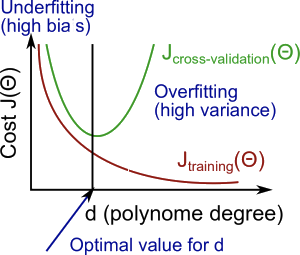
\includegraphics[scale=0.4]{./images/bias_and_variance_polynomial.png}
\end{center}

\noindent High bias(underfitting): both \(J_{train}(W, B)\) and \(J_{cv}(W, B)\) will be high. Also, \(J_{cv}(W, B) \approx J_{train}(W, B)\). 

\noindent High variance(overfitting): \(J_{train}(W, B)\) will be low and \(J_{cv}(W, B)\) will be high. Also, \(J_{cv}(W, B) \gg J_{train}(W, B)\). 

\bigskip

\noindent \textbf{underfitting}:

\noindent High bias, which means hypothesis fits training data poorly, is usually caused by a function that is too simple or using too few features. 

\bigskip

\noindent \textbf{overfitting}:

\noindent High variance, which means hypothesis fits training data well, but does not generalize well to predict new data. It is usually caused by a complicated function with too many features.

\subsection{Basic Recipe for Machine Learning}

\noindent If your algorithm has a high bias:

\begin{itemize}
  \item Try to make your NN bigger (size of hidden units, number of layers)
  \item Try a different model (architecture) that is suitable for your data.
  \item Try to run it longer.
  \item Different (advanced) optimization algorithms.
\end{itemize}

\noindent If your algorithm has a high variance:

\begin{itemize}
  \item More data.
  \item Try regularization.
  \item Try a different model (architecture) that is suitable for your data.
\end{itemize}

\noindent You should try the previous two points until you have a low bias and low variance. In the older days before deep learning, there was a "Bias/variance tradeoff". But because now you have more options/tools for solving the bias and variance problem its really helpful to use deep learning. With enough training data, training a bigger neural network never hurts.

\bigskip

\noindent \textbf{Regularization}: (L2 Regularization) 

\noindent Add regularization term to the cost function to reduce variance (overfitting):

\[\frac{\lambda}{2m} \sum_{l = 1}^{L} \sum_{i = 1}^{s_l} \sum_{j = 1}^{s_{l + 1}} (W_{j, i}^{[l]})^{2} = \frac{\lambda}{2m} np.sum(W \odot W)\]

\bigskip

\noindent weight backpropagation with regularization:

\[W^{[l]} := W^{[l]} - \alpha \partial W^{[l]} = (1 - \frac{\alpha \lambda}{m}) W^{[l]} - \frac{\alpha}{m} \partial Z^{[l]} (A^{[l - 1]})^T\]

\noindent The new term \((1 - \frac{\alpha \lambda}{m}) W^{[l]}\) causes the weight to decay in proportion to its size. In practice this penalizes large weights and effectively limits the freedom in your model.


\begin{itemize}
  \item If \(\lambda\) is too large - \(W^{[l]}_{i,j}\) will be close to zeros which will make the NN simpler.
  \item If \(\lambda\) is good enough it will just reduce some weights and prevent the overfitting.
  \item If \(\lambda\) is too large, \(Z^{[l]}_{i}\) will be small (close to zero) - assume tanh activation function is used, then it will behave like a linear function, so we will go from non linear activation to roughly linear which would make the NN a roughly linear classifier.
  \item If \(\lambda\) good enough it will just make some of tanh activations roughly linear which will prevent overfitting.
\end{itemize}

\noindent Implementation tip: if you implement gradient descent, plot the cost function as a function of the number of iterations of gradient descent and you want to see that the cost function decreases monotonically after every elevation of gradient descent with regularization.

\bigskip

\noindent \textbf{Dropout}:

\noindent The dropout regularization eliminates some neurons/weights on each iteration based on a probability. It is used to reduce overfitting. A most common technique to implement dropout is called "Inverted dropout".

\[keep\_prob = 0.8 \text{ (for example)}\]
\[D^{[l]} = np.random.rand(A^{[l]}.shape[0], A^{[l]}.shape[1]) < keep\_prob\]
\[A^{[l]} = A^{[l]} \odot D^{[l]}\]
\[A^{[l]} = keep\_prob^{-1} A^{[l]}\]

\begin{center}
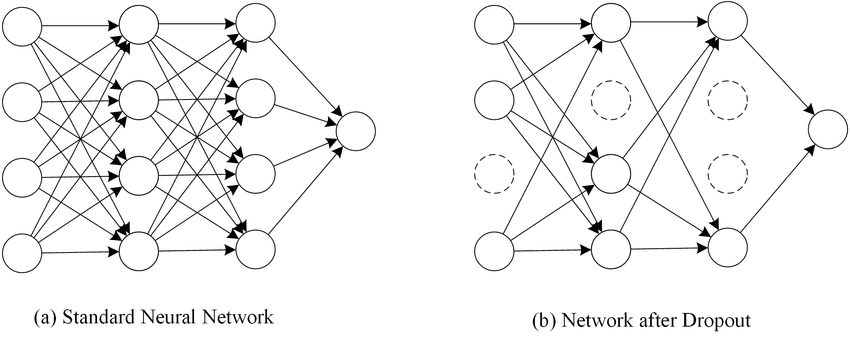
\includegraphics[scale=0.4]{./images/dropout_neural_network.png}
\end{center}

\noindent Drop 20\% of units in \(A^{[l]}\) by replacing them with 0, then scale \(A^{[l]}\) by \(keep\_prob^{-1}\). 

\bigskip

\noindent We need to scale \(A^{[l]}\) because \(Z^{[l + 1]} = W^{[l + 1]} A^{[l]} + B^{[l + 1]}\). And we want to increase \(A^{[l]}\) to not reduce the expected value of output \(Z^{[l + 1]}\) after dropout.

\bigskip

\noindent \(D^{[l]}\) is used for forward and back propagation and is the same for them, but it is different for each iteration of training example. At test time we don't use dropout. Otherwise it would add noise to predictions.

\bigskip

\noindent \textbf{Understanding Dropout}:

\begin{itemize}
  \item The intuition is dropout randomly knocks out units in your network. So it's as if on every iteration you're working with a smaller NN, and so using a smaller NN seems like it should have a regularizing effect.
  \item Another intuition: can't rely on any single feature, so have to spread out weights.
  \item Dropout can have different keep\_prob per layer.
  \item The input layer dropout has to be near 1 (or 1 - no dropout) because you don't want to eliminate a lot of features.
  \item If you're more worried about some layers overfitting than others, you can set a lower keep\_prob for some layers than others. The downside is, this gives you even more hyperparameters to search for using cross-validation. One other alternative might be to have some layers where you apply dropout and some layers where you don't apply dropout and then just have one hyperparameter, which is a keep\_prob for the layers for which you do apply dropouts.
  \item A lot of researchers are using dropout with Computer Vision (CV) because they have a very big input size and almost never have enough data, so overfitting is the usual problem.
  \item A downside of dropout is that the cost function is not well defined and it will be hard to debug (plot cost by iteration). To solve that you'll need to turn off dropout, set all the keep\_prob to 1, and then run the code and check that it monotonically decreases cost and then turn on the dropouts again.
\end{itemize}

\noindent \textbf{Other regularization methods}:

\begin{itemize}
  \item Data augmentation. For example, you can flip all your pictures horizontally this will give you m more data instances. You could also apply a random position and rotation to an image to get more data. New data obtained using this technique isn't as good as the real independent data, but still can be used as a regularization technique.
  \item Early stopping. We will pick the point at which the training set error and dev set error are best (lowest training cost with lowest dev cost). We will take these parameters as the best parameters.
\end{itemize}

\noindent \textbf{Normalizing Inputs}: (Feature Scaling)

\noindent All features should be normalized so that they are scaled into a certain range and each feature contributes approximately proportionately to the result. It helps to center the dataset. Also it helps gradient descent converge much faster.

\bigskip

\noindent This should be applied to training, dev, and testing sets (but using mean and variance of the training set).

\begin{center}
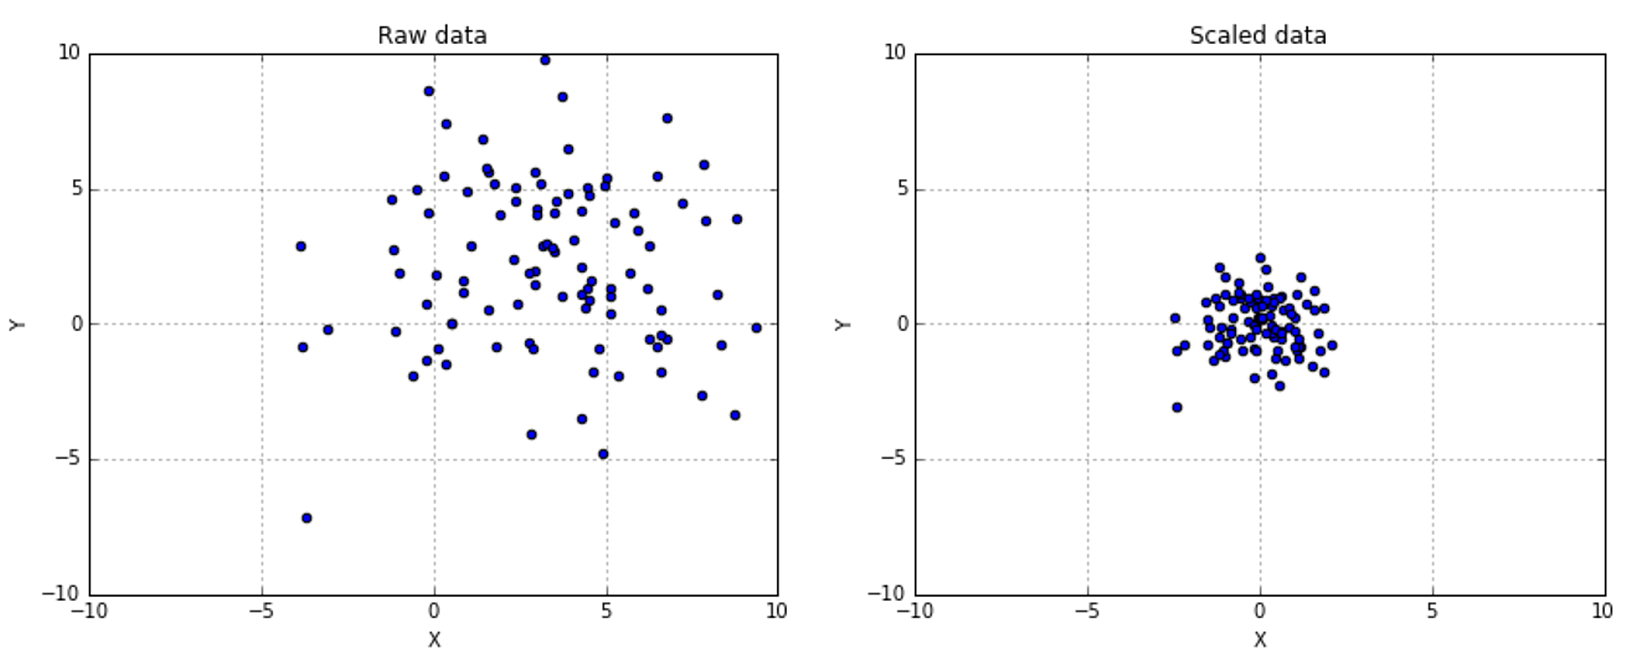
\includegraphics[scale=0.8]{./images/normalize_input.png}
\end{center}

\noindent If we normalize inputs, the shape of the cost function will be consistent (look more symmetric like circle in 2D example) and we can use a larger learning rate alpha - the optimization will be faster.

\begin{center}
\includegraphics[scale=0.4]{./images/normalize_cost.png}
\end{center}

\bigskip

\noindent \textbf{mean normalization}:

\[x_i = \frac{x_i - mean(x_i)}{max(x_i) - min(x_i)}\]

\bigskip

\noindent \textbf{standardization}:

\noindent Feature standardization makes the values of each feature in the data have zero-mean (when subtracting the mean in the numerator) and unit-variance.

\[\mu: \text{mean, } \sigma^2: \text{variance, } \sigma: \text{standard deviation}\]

\[\mu_i ={\frac {1}{m}}\sum _{j=1}^{m}x^{(j)}_{i}\]

\[\sigma^2_i = \frac{1}{m} \sum_{j = 1}^m (x^{(j)}_i - \mu_i)^2\]

\[x_i = \frac{x_i - \mu_i}{\sigma_i}\]

\noindent \textbf{Gradient Vanishing/Exploding}:

\noindent In a deep neural network, when the weights or derivatives for each layer get a little bit smaller/larger, the final gradient could be exponentially smaller/larger with respect to \(L\). Too small/large gradient could cause weights update overshot or in tiny steps, and make training process unable to continue.

\bigskip

\noindent \textbf{Weight Initialization}:

\noindent A partial solution to the Vanishing / Exploding gradients is better or more careful choice of the random initialization of weights. 

\bigskip

\noindent Some researcher found that: (He Initialization / Xavier Initialization)

\bigskip

\noindent If \(tanh\) is used as activation function, the variance of \(W^{[l]}\) should be \(\frac{1}{s_{l - 1}}\), then \(W^{[l]}\) should be initialized as:

\[W^{[l]} = np.random.randn(s_{l - 1}, s_l) * np.sqrt(\frac{1}{s_{l - 1}}) \]

\noindent If \(relu\) is used as activation function, the variance of \(W^{[l]}\) should be \(\frac{2}{s_{l - 1}}\), then \(W^{[l]}\) should be initialized as:

\[W^{[l]} = np.random.randn(s_{l - 1}, s_l) * np.sqrt(\frac{2}{s_{l - 1}}) \]

\noindent Some old paper use this as well:

\[W^{[l]} = np.random.randn(s_{l - 1}, s_l) * np.sqrt(\frac{2}{s_{l - 1} + s_{l}}) \]

\noindent \textbf{Gradient checking:}

\noindent Compose \(W\), \(B\) into one big vector \(\Theta\). We can approximate the derivative of \(J(\Theta)\) with respect to \(\Theta_{i}\) as:

\[\frac{\partial}{\partial \Theta_{i}} J(\Theta) \approx \frac{J(\dots, \Theta_{i} + \epsilon, \dots) - J(\dots, \Theta_{i} - \epsilon, \dots)}{2\epsilon}\]

\noindent A small value for \(\epsilon\) such as \(\epsilon = 10^{-7}\), guarantees that the math works out properly. If the value for \(\epsilon\) is too small, we can end up with numerical problems. Then we can check if \(gradApprox \approx deltaVector\).

\begin{itemize}
  \item if it is \(< 10^{-7}\) - great, very likely the backpropagation implementation is correct
  \item if around \(10^{-5}\) - can be OK, but need to inspect if there are no particularly big values in \(d\_theta\_approx - d\_theta\) vector
  \item if it is \(> 10^{-3}\) - bad, probably there is a bug in backpropagation implementation
\end{itemize}

\noindent gradient checking implementation notes:

\begin{itemize}
  \item Don't use the gradient checking algorithm at training time because it's very slow. Use gradient checking only for debugging.
  \item If algorithm fails grad check, look at components to try to identify the bug.
  \item Don't forget to add regularization term to \(J(W, B)\) if you are using L1 or L2 regularization.
  \item Gradient checking doesn't work with dropout because cost function is not consistent. You can first turn off dropout \(keep\_prob = 1.0\), run gradient checking and then turn on dropout again.
  \item Run gradient checking at random initialization and train the network for a while maybe there's a bug which can be seen when w's and b's become larger (further from 0) and can't be seen on the first iteration (when w's and b's are very small).
\end{itemize}

\noindent \textbf{Mini-batch gradient descent}:

\noindent When training set is getting too big, it is impossible to use entire training set \(X\), \(Y\) to do a vectorized gradient descent. Instead we can separate the training set into mini batches, and do a vectorized gradient descent for each of them at a time.

\bigskip

\noindent After we iterate through the entire training set (all batches) for one time, we call it an \(epoch\). The model should be trained for enough \(epochs\) until the cost function converges.

\bigskip

\noindent Suppose we have \(m\) training examples, and we use \(batch\_size = 1000\), then we have \(num\_batches = \frac{m}{batch\_size}\). The mini batches are \(X^{\{t\}}\), \(Y^{\{t\}}\) for \(t \in [1, num\_batches]\). And we want to train the model with entire training set for \(num\_epochs = 10000\) times.

\bigskip

\noindent \textbf{mini-batch gradient descent algorithm}:

\noindent for \(epoch \in \{1, \dots, num\_epochs\}\):

\noindent \hspace{.5cm} for \(t \in \{1, \dots, num\_batches\}\):

\noindent \hspace{1cm} vectorized gradient descent with mini batch \(X^{\{t\}}\), \(Y^{\{t\}}\):

\noindent \hspace{1cm} \(W =: W - \alpha \partial W\)

\noindent \hspace{1cm} \(B =: B - \alpha \partial B\)

\bigskip

\noindent \textbf{Understanding Mini-Batch Gradient Descent}:

\noindent In mini-batch algorithm, the cost won't go down with each step as it does in batch algorithm (not enough training data in one mini batch, not as effective as batch algorithm). It could contain some ups and downs but generally it has to go down (unlike the batch gradient descent where cost function decreases on each iteration).

\begin{itemize}
  \item \(batch\_size = m\), Batch gradient descent, too long per iteration
  \item \(batch\_size = 1\), Stochastic gradient descent (SGD), too noisy regarding cost minimization (can be reduced by using smaller learning rate), won't ever converge (reach the minimum cost), lose speedup from vectorization
  \item \(batch\_size \in [1, m]\), Mini-batch gradient descent, have the vectorization advantage, make progress without waiting to process the entire training set, doesn't always exactly converge (oscillates in a very small region, but you can reduce learning rate)
\end{itemize}

\begin{center}
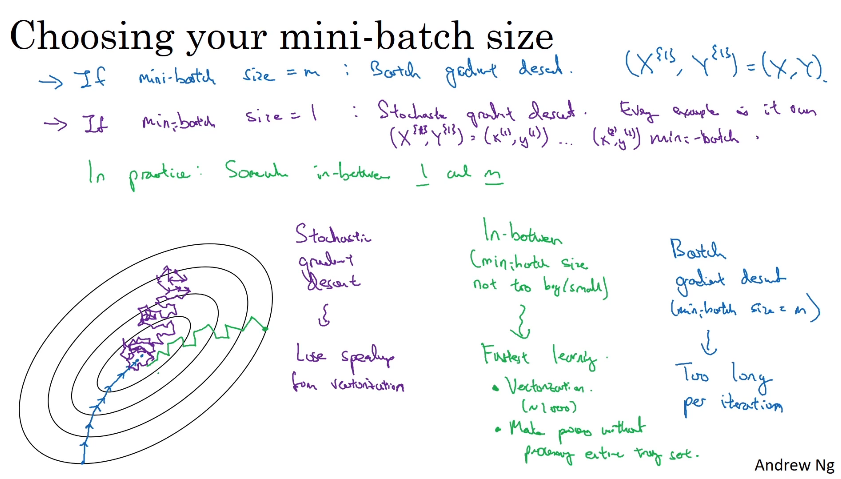
\includegraphics[scale=0.4]{./images/mini_batch.png}
\end{center}

\noindent \textbf{Guidelines for choosing mini-batch size}:

\begin{itemize}
  \item If small training set - use batch gradient descent.
  \item It has to be a power of 2 (because of the way computer memory is Laid out and accessed, sometimes your code runs faster): \(2^{6}, 2^{7}, 2^{8}, 2^{9}, 2^{10} \dots\)
  \item Make sure that mini-batch fits in CPU/GPU memory.
  \item Mini-batch size is a hyperparameter.
\end{itemize}

\subsection{Exponentially Weighted Averages}

\begin{center}
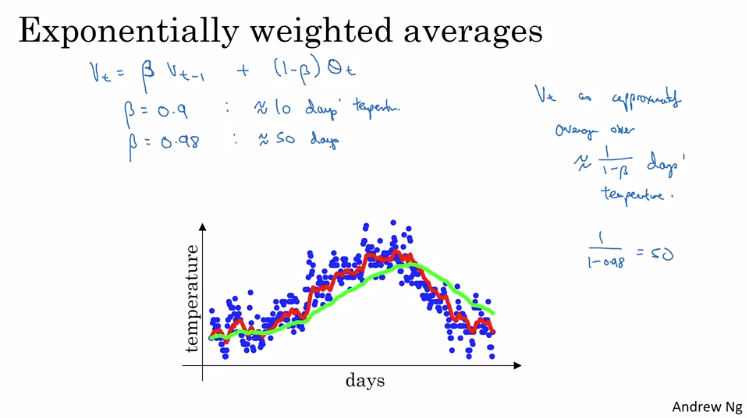
\includegraphics[scale=0.4]{./images/exponentially_weighted_average.png}
\end{center}

\noindent If we have a daily temperature list like this:

\[\theta_{1} = 40, \theta_{2} = 49, \theta_{3} = 45, \dots, \theta_{50} = 56\]

\noindent We call \(v_{t}\) is the exponentially weighted average of daily temperature over the last \(\frac{1}{1 - \beta}\) days: (\(\beta \in [0, 1)\))

\[v_{0} = 0\]
\[v_{1} = \beta v_{0} + (1 - \beta) \theta_{1}\]
\[v_{2} = \beta v_{1} + (1 - \beta) \theta_{2}\]
\[\dots\]
\[v_{t} = \beta v_{t - 1} + (1 - \beta) \theta_{t}\]

\noindent \textbf{Bias Correction of Exponentially Weighted Averages}:

\noindent The bias correction helps make the exponentially weighted averages more accurate. Because \(v_{0} = 0\), the initial weighted averages are too small and the accuracy suffers at the start. To fix the bias for the initial estimates we have to use this equation: (As \(t\) becomes larger the \(1 - \beta^{t}\) becomes close to 1)

\[v_{t} = \frac{\beta v_{t - 1} + (1 - \beta) \theta_{t}}{1 - \beta^{t}}\]

\subsection{Gradient Descent With Momentum}

\noindent The momentum algorithm almost always works faster than standard gradient descent. It smooths out the steps of gradient descent by using the exponentially weighted average of the gradients. In practice people don't bother implementing bias correction.

\begin{center}
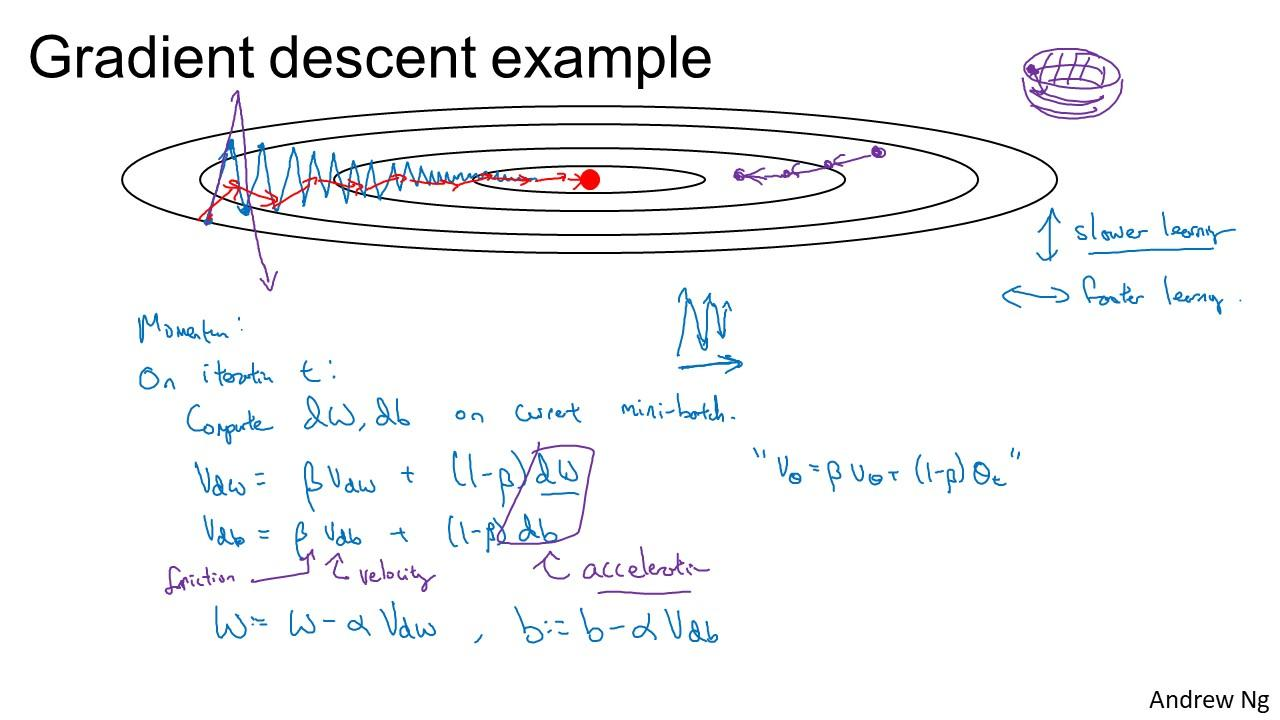
\includegraphics[scale=0.2]{./images/momentum_gradient_descent.jpg}
\end{center}

\noindent \textbf{gradient descent with momentum}:

\noindent \(v_{\partial W} = 0, v_{\partial B} = 0\)

\noindent for \(epoch \in \{1, \dots, num\_epochs\}\):

\noindent \hspace{.5cm} for \(t \in \{1, \dots, num\_batches\}\):

\noindent \hspace{1cm} vectorized gradient descent with mini batch \(X^{\{t\}}\), \(Y^{\{t\}}\):

\noindent \hspace{1cm} \(v_{\partial W} =: \beta v_{\partial W} + (1 - \beta) \partial W\)

\noindent \hspace{1cm} \(v_{\partial B} =: \beta v_{\partial B} + (1 - \beta) \partial B\)

\noindent \hspace{1cm} \(W =: W - \alpha v_{\partial W}\)

\noindent \hspace{1cm} \(B =: B - \alpha v_{\partial B}\)

\subsection{RMSProp(Root mean square prop)}

\noindent RMSprop can speed up the gradient descent by dividing the gradient \(\partial W\), \(\partial B\) by a manually constructed term: If gradient is small, divided by a small term will make it larger, and make gradient descent faster in this direction; If gradient is large, divided by a large term will make it smaller, and make gradient descent slower in this direction.

\bigskip

\noindent It will make the cost function move slower on the vertical direction and faster on the horizontal direction in the following example:

\begin{center}
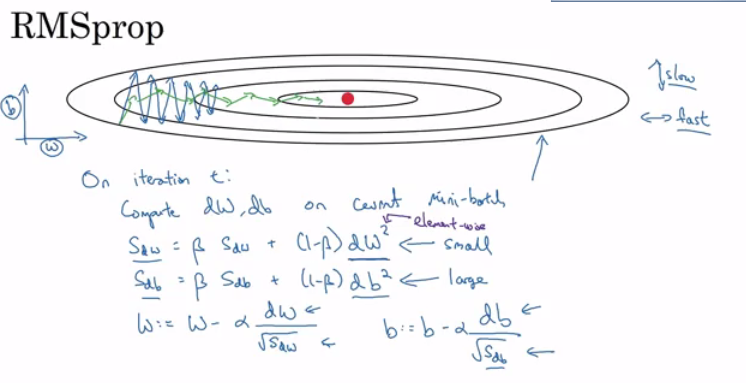
\includegraphics[scale=0.4]{./images/RMSprop.png}
\end{center}

\noindent \textbf{RMSProp}:

\noindent \(s_{\partial W} = 0, s_{\partial B} = 0\)

\noindent make sure denominator is not too small: \(\epsilon = 10^{-8}\)

\noindent for \(epoch \in \{1, \dots, num\_epochs\}\):

\noindent \hspace{.5cm} for \(t \in \{1, \dots, num\_batches\}\):

\noindent \hspace{1cm} vectorized gradient descent with mini batch \(X^{\{t\}}\), \(Y^{\{t\}}\):

\noindent \hspace{1cm} \(s_{\partial W} =: \beta s_{\partial W} + (1 - \beta) \partial W \odot \partial W\)

\noindent \hspace{1cm} \(s_{\partial B} =: \beta s_{\partial B} + (1 - \beta) \partial B \odot \partial B\)

\noindent \hspace{1cm} \(W =: W - \alpha \frac{\partial W}{\sqrt{s_{\partial W}} + \epsilon}\)

\noindent \hspace{1cm} \(B =: B - \alpha \frac{\partial B}{\sqrt{s_{\partial B}} + \epsilon}\)

\subsection{Adam Optimization Algorithm}

\noindent Adam (Adaptive Moment Estimation) optimization algorithm combined momentum and RMSProp methods. Hyperparameters for Adam:

\begin{itemize}
    \item \(\alpha\): learning rate
    \item \(\beta_{1}\): parameter of the momentum - 0.9 is recommended by default.
    \item \(\beta_{2}\): parameter of the RMSprop - 0.999 is recommended by default.
    \item \(\epsilon\): \(10^{-8}\) is recommended by default.
\end{itemize}

\noindent \textbf{adam optimization algorithm}:

\noindent \(v_{\partial W} = 0, v_{\partial B} = 0, s_{\partial W} = 0, s_{\partial B} = 0\)

\noindent make sure denominator is not too small: \(\epsilon = 10^{-8}\)

\noindent for \(epoch \in \{1, \dots, num\_epochs\}\):

\noindent \hspace{.5cm} for \(t \in \{1, \dots, num\_batches\}\):

\noindent \hspace{1cm} vectorized gradient descent with mini batch \(X^{\{t\}}\), \(Y^{\{t\}}\):

\noindent \hspace{1cm} \(v_{\partial W} =: \beta_{1} v_{\partial W} + (1 - \beta_{1}) \partial W\)

\noindent \hspace{1cm} \(v_{\partial B} =: \beta_{1} v_{\partial B} + (1 - \beta_{1}) \partial B\)

\noindent \hspace{1cm} \(s_{\partial W} =: \beta_{2} s_{\partial W} + (1 - \beta_{2}) \partial W \odot \partial W\)

\noindent \hspace{1cm} \(s_{\partial B} =: \beta_{2} s_{\partial B} + (1 - \beta_{2}) \partial B \odot \partial B\)

\noindent \hspace{1cm} \(v^{corrected}_{\partial W} =: \frac{v_{\partial W}}{1 - \beta^{t}_{1}}\)

\noindent \hspace{1cm} \(v^{corrected}_{\partial B} =: \frac{v_{\partial B}}{1 - \beta^{t}_{1}}\)

\noindent \hspace{1cm} \(s^{corrected}_{\partial W} =: \frac{s_{\partial W}}{1 - \beta^{t}_{2}}\)

\noindent \hspace{1cm} \(s^{corrected}_{\partial B} =: \frac{s_{\partial B}}{1 - \beta^{t}_{2}}\)

\noindent \hspace{1cm} \(W =: W - \alpha \frac{v^{corrected}_{\partial W}}{\sqrt{s^{corrected}_{\partial W}} + \epsilon}\)

\noindent \hspace{1cm} \(B =: B - \alpha \frac{v^{corrected}_{\partial B}}{\sqrt{s^{corrected}_{\partial B}} + \epsilon}\)

\subsection{Learning Rate Decay}

Slowly reduce learning rate for each epoch helps cost function to converge near the optimum point.

\begin{center}
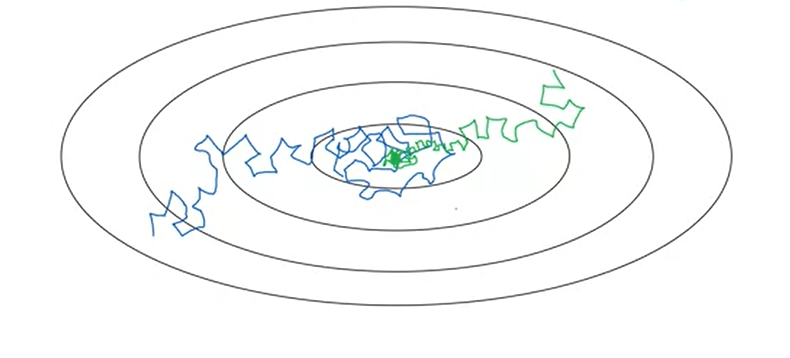
\includegraphics[scale=0.4]{./images/learning_rate_decay.png}
\end{center}

\noindent \textbf{learning rate decay}:

\noindent initial learning rate: \(\alpha_{0}\), decay rate: \(d\)

\noindent for each epoch \(p\): \(\alpha_{p} = \frac{1}{1 + d \times p} \alpha_{0}\)

\bigskip

\noindent \textbf{other learning rate decay}:

\begin{itemize}
    \item exponentially decay: \(\alpha_{p} = o.95^{p} \alpha_{0}\)
    \item \(\alpha_{p} = \frac{k}{\sqrt{p}} \alpha_{0}\) or \(\alpha_{t} = \frac{k}{\sqrt{t}} \alpha_{0}\)
    \item manually learning rate decay.
\end{itemize}

\subsection{Tuning Process}

\noindent Hyperparameters priority: (as for Andrew Ng)

\begin{itemize}
    \item \(\alpha\)
    \item \(\beta\)
    \item \(s_{l}\)
    \item \(batch\_size\)
    \item \(L\)
    \item \(d\)
    \item \(\beta_{1}, \beta_{2}, \epsilon\)
\end{itemize}

\noindent Tune Hyperparameters:

\begin{itemize}
    \item give each Hyperparameter a range
    \item randomly pick a value for each Hyperparameter in its range, then train with them
    \item randomly picking helps to explore Hyperparameters in a larger range (compare with increasing by steps), which can give hints to narrow the range and speed up the tuning process
    \item use Coarse to fine sampling scheme: when you find some hyperparameter values that give you a better performance - zoom into a smaller region around these values and sample more densely within this space
\end{itemize}

\noindent \textbf{Using scale to pick hyperparameters}

\noindent Let's say you have a specific wide range for a hyperparameter from "a" to "b". It's better to search for the right ones using the logarithmic scale rather then in linear scale:

\[a = -4, b = 0\]
\[r \in [a, b]\]
\[r = -4 \times np.random.rand()\]
\[\alpha = 10^{r}\]

\noindent \textbf{Panda vs. Caviar}

\noindent Intuitions about hyperparameter settings from one application may or may not transfer to a different one.

\begin{itemize}
    \item If you don't have much computational resources you can use the "babysitting model" (Panda Approach): Day 0 you might initialize your parameter as random and then start training. Then you watch your learning curve gradually decrease over the day. And each day you nudge your parameters a little during training.
    \item If you have enough computational resources, you can run several models in parallel and at the end of the day(s) you check the results (Caviar Approach).
\end{itemize}

\noindent \textbf{Batch Normalization}:

\noindent \noindent Normalized inputs could be shifted in the hidden layers. Batch normalization reduces the problem of input values changing (shifting). And it speeds up learning as well. In practice, normalizing \(Z^{[l]}\) is done much more often and that is what Andrew Ng presents.

\bigskip

\noindent For a layer \(l\), given a mini batch of samples \(Z^{[l](1)}, \dots, Z^{[l](m)}\):

\[\mu = \frac{1}{m} \sum^{m}_{i = 1} Z^{[l](i)}\]
\[\sigma^{2} = \frac{1}{m} \sum^{m}_{i = 1} (Z^{[l](i)} - \mu) \odot (Z^{[l](i)} - \mu)\]
\[Z^{[l](i)}_{norm} = (Z^{[l](i)} - \mu) \oslash \sqrt{\sigma^{2} + \epsilon}\]
\[\overset{N}{Z}^{[l](i)} = \gamma^{[l]} \odot Z^{[l](i)}_{norm} + \beta^{[l]}\]

\noindent \(\epsilon\) is added for numerical stability (in case \(\sigma\) is too small). \(\gamma, \beta\) are learnable parameters of the model, and they make inputs belong to other distribution (with other mean and variance). It makes the NN learn the distribution of the outputs.

\bigskip

\noindent Batch normalization does some regularization:

\begin{itemize}
    \item Each mini batch is scaled by the mean/variance computed of that mini-batch.
    \item This adds some noise to the values \(Z^{[l]}\) within that mini batch. So similar to dropout it adds some noise to each hidden layer's activations.
\end{itemize}

\noindent \textbf{Gradient Descent with Batch Normalization}:

\noindent (also can work with Momentum, RMSprop, Adam...)

\noindent for \(epoch \in \{1, \dots, num\_epochs\}\):

\noindent \hspace{.5cm} for \(t \in \{1, \dots, num\_batches\}\):

\noindent \hspace{1cm} vectorized gradient descent with mini batch \(X^{\{t\}}\), \(Y^{\{t\}}\):

\noindent \hspace{1cm} use \(\overset{N}{Z}^{\{t\}}\) to replace \(Z^{\{t\}}\)

\noindent \hspace{1cm} \(B\) will be replaced by \(\beta\)

\noindent \hspace{1cm} \(W =: W - \alpha \partial W\)

\noindent \hspace{1cm} \(\gamma =: \gamma - \alpha \partial \gamma\)

\noindent \hspace{1cm} \(\beta =: \beta - \alpha \partial \beta\)

\bigskip

\noindent \textbf{Batch normalization at test time}:

\noindent When we train a NN with Batch normalization, we compute the mean and the variance of the mini-batch. In testing we might need to process examples one at a time. The mean and the variance of one example won't make sense. We have to compute an estimated value of mean and variance to use it in testing time. We can use the exponentially weighted average of \(\mu, \sigma^{2}\) across the mini-batches. In practice most often you will use a deep learning framework and it will contain some default implementation of doing such a thing.

\bigskip

\noindent Given \(t\) mini batches of training examples:

\noindent \(\mu_{test}\) is exponentially weighted average of \(\mu^{\{1\}}, \mu^{\{2\}}, \dots, \mu^{\{t\}}\)

\noindent \(\sigma^{2}_{test}\) is exponentially weighted average of \(\sigma^{2\{1\}}, \sigma^{2\{2\}}, \dots, \sigma^{2\{t\}}\)

\[Z_{norm} = (Z - \mu_{test}) \oslash \sqrt{\sigma^{2}_{test} + \epsilon}\]
\[\overset{N}{Z} = \gamma \odot Z_{norm} + \beta\]

\noindent \textbf{Softmax Regression}:

\noindent Softmax regression is used for multiclass classification/regression. It is normally used in the last layer. Each of values in the output layer represents a probability of the example to belong to each of the classes, and they sum up to 1.

\[t = e^{Z^{[L]}}\]
\[A^{[L]} = \frac{t}{sum\{t\}}\]

\noindent \textbf{Train with Softmax}:

\noindent With machine learning framework like Tensorflow, Forward Propagation needs to be built, Backpropagation part can be handled automatically .

\[L(\hat{y}, y) = - \sum^{K}_{k = 1} y_{k}log(\hat{y}_{k}) \]
\[J(W, B) = - \frac{1}{m} \sum_{i = 1}^{m} L(\hat{y}^{(i)}, y^{(i)})\]
\[\partial Z^{[L]} = \hat{y} - y\]
\[\partial Z^{[l]} = \dots\]

\noindent \textbf{Local Optima}:

\begin{itemize}
    \item The normal local optima is not likely to appear in a deep neural network because data is usually high dimensional. For point to be a local optima it has to be a local optima for each of the dimensions which is highly unlikely.
    \item It's unlikely to get stuck in a bad local optima in high dimensions, it is much more likely to get to the saddle point rather to the local optima, which is not a problem.
    \item Plateaus can make learning slow. Plateau is a region where the derivative is close to zero for a long time. This is where algorithms like momentum, RMSprop or Adam can help.
\end{itemize}

\section{Structuring Machine Learning Projects}

\subsection{Orthogonalization}

\noindent Some deep learning developers know exactly what hyperparameter to tune in order to try to achieve one effect. This is a process we call orthogonalization. In orthogonalization, you have some controls, but each control does a specific task and doesn't affect other controls.

\bigskip

\noindent For a supervised learning system to do well, you usually need to tune the knobs of your system to make sure that four things hold true - chain of assumptions in machine learning:

\begin{itemize}
    \item You'll have to fit training set well on cost function (near human level performance if possible). If it's not achieved you could try bigger network, another optimization algorithm (like Adam)...
    \item Fit dev set well on cost function. If its not achieved you could try regularization, bigger training set...
    \item Fit test set well on cost function. If its not achieved you could try bigger dev set...
    \item Performs well in real world. If its not achieved you could try change dev set, change cost function...
\end{itemize}

\subsection{Single Number Evaluation Metric}

\noindent \textbf{Precision \& Recall: (deal with skewed classes)}

\noindent High \(F_{score} \in [0, 1]\) (high precision and high recall) represents a good prediction model. (use average value of precision and recall for all classes if there are multiple classes)

\begin{center}
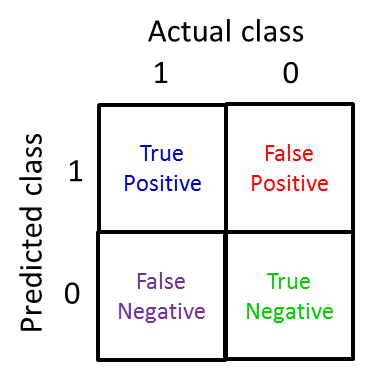
\includegraphics[scale=0.6]{./images/precision_recall.png}
\end{center}

\[\text{Precision} = \frac{\text{True positives}}{\text{predicted as positive}} = \frac{\text{True positives}}{\text{True positives + False positives}}\]
\[\text{Recall} = \frac{\text{True positives}}{\text{actual positives}} = \frac{\text{True positives}}{\text{True positives + False negatives}}\]
\[F_{score} = \frac{2}{\frac{1}{\text{Precision}} + \frac{1}{\text{Recall}}} = 2 \times \frac{\text{Precision} \times \text{Recall}}{\text{Precision + Recall}}\]

\noindent \textbf{Satisficing and Optimizing Metrics}:

\noindent Assume we have \(N\) metrics to evaluate the model, normally we will have \(1\) optimizing metric, and \(N - 1\) satisficing metrics. For example: Maximize optimizing metric \(F_{score}\), subject to satisficing metrics \(RunningTime < 100ms\), \(ModelSize < 1gb\).

\subsection{Train/Dev/Test Set Distributions}

Dev and test sets have to come from the same distribution. Choose dev set and test set to reflect data you expect to get in the future and consider important to do well on. Setting up the dev set, as well as the validation metric is really defining what target you want to aim at.

\bigskip

\noindent \textbf{Size of the dev and test sets}:

\noindent An old way of splitting the data was 70\% training, 30\% test or 60\% training, 20\% dev, 20\% test. The old way was valid for a number of examples \(< 100000\) In the modern deep learning if you have a million or more examples a reasonable split would be 98\% training, 1\% dev, 1\% test.

\bigskip

\noindent \textbf{When to change dev/test sets and metrics}:

\noindent Orthogonalization for deep learning: break a machine learning problem into distinct steps.

\begin{itemize}
    \item Figure out how to define a metric that captures what you want to do - place the target.
    \item Worry about how to actually do well on this metric - how to aim/shoot accurately at the target.
\end{itemize}

\noindent Conclusion: if doing well on your metric + dev/test set doesn't correspond to doing well in your application, change your metric and/or dev/test set.

\subsection{Human-level Performance}

\noindent We compare to human-level performance because of two main reasons:

\begin{itemize}
    \item Because of advances in deep learning, machine learning algorithms are suddenly working much better and so it has become much more feasible in a lot of application areas for machine learning algorithms to actually become competitive with human-level performance.
    \item It turns out that the workflow of designing and building a machine learning system is much more efficient when you're trying to do something that humans can also do.
\end{itemize}

\noindent After an algorithm reaches the human level performance the progress and accuracy slow down.

\begin{center}
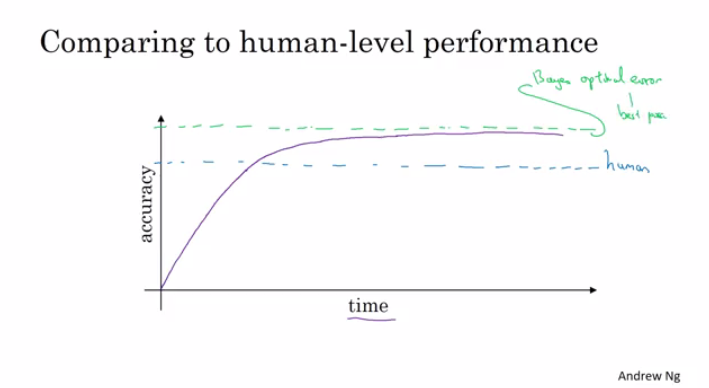
\includegraphics[scale=0.6]{./images/human_level_performance.png}
\end{center}

\noindent You won't surpass an error that's called "Bayes optimal error" (the minimum possible error that can be made). There isn't much error range between human-level error and Bayes optimal error.

\bigskip

\noindent Humans are quite good at a lot of tasks. So as long as Machine learning is worse than humans, you can:

\begin{itemize}
    \item Get labeled data from humans.
    \item Gain insight from manual error analysis: why did a person get it right?
    \item Better analysis of bias/variance.
\end{itemize}

\noindent \textbf{Avoidable bias}:

\noindent Suppose that the cat classification algorithm gives these results:

\begin{center}
\begin{tabular}{ |c|c|c| } 
 \hline
 Humans & 1\% & 7.5\% \\ 
 \hline
 Training error & 8\% & 8\% \\ 
 \hline
 Dev Error & 10\% & 10\%	 \\ 
 \hline
\end{tabular}
\end{center}

\noindent The human-level error as a proxy (estimate) for Bayes optimal error. Bayes optimal error is always less (better), but human-level in most cases is not far from it. You can't do better than Bayes error unless you are overfitting.

\[\text{Avoidable Bias} = \text{Training error} - \text{Human (Bayes) error}\]
\[\text{Measure of Variance} = \text{Dev error} - \text{Training error}\]

\noindent In the left example, because the Avoidable Bias is larger (7\%) then we need to focus on the bias. In the right example, because the Measure of Variance is larger (2\%) then we need to focus on the variance.

\bigskip

\noindent You might have multiple human-level performances based on different groups of people. Choose the best human-level performance as it is closer to Bayes optimal error.

\bigskip

\noindent These techniques allow you to make decisions more quickly as to whether you should focus on trying to reduce the bias or trying to reduce the variance of your algorithm. This tend to work well until you surpass human-level performance, whereupon you might no longer have a good estimate of Bayes error that still helps you make this decision really clearly.

\bigskip

\noindent \textbf{Surpassing human-level performance}:

\noindent In some problems, deep learning has surpassed human-level performance. Like:

\begin{itemize}
    \item Online advertising.
    \item Product recommendation.
    \item Logistics (predict transit time)
    \item Loan approval.
\end{itemize}

\noindent These examples are learning on structural data with lots of data, and they are not natural perception task. Humans behave well in natural perception tasks like medical, computer vision and speech recognition, and it's harder to surpass human-level performance in these tasks.

\subsection{Error analysis}

\noindent Error analysis - process of manually examining mistakes that your algorithm is making. It can give you insights into what to do next. Error analysis helps you to analyze the error before taking an action which could take unnecessary efforts.

\bigskip

\noindent Sometimes, you can evaluate multiple error analysis ideas in parallel and choose the best idea, by creating a spreadsheet of them. This quick counting procedure, which takes small numbers of hours, can really help you make much better prioritization decisions, and understand how promising different approaches are to work on.

\begin{center}
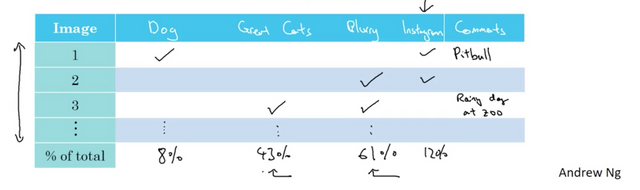
\includegraphics[scale=0.5]{./images/error_analysis.png}
\end{center}

\noindent \textbf{Incorrectly Labeled Data}:

\noindent DL algorithms are quite robust to random errors in the training set but less robust to systematic errors. Only fix these labels for training set if you can. If you want to check for mislabeled data in dev/test set, try error analysis with the mislabeled column.

\begin{center}
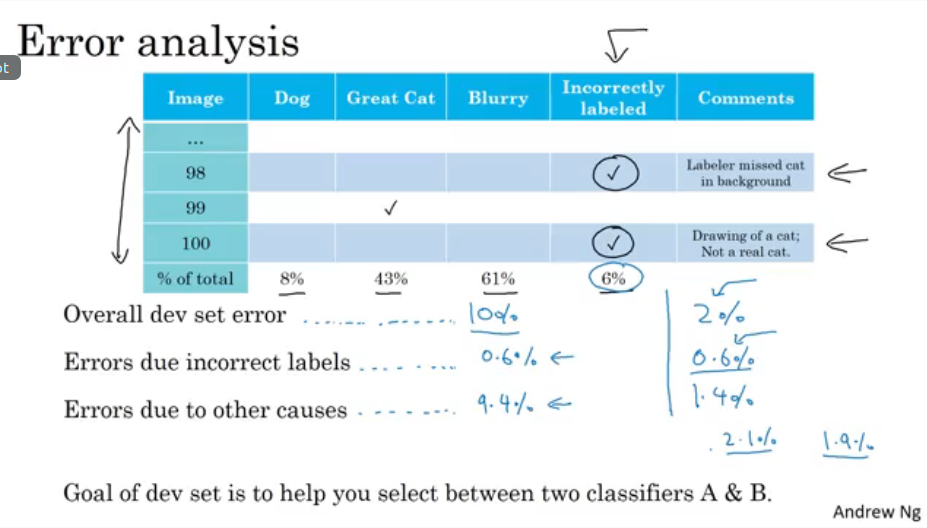
\includegraphics[scale=0.4]{./images/incorrectly_labeled_data.png}
\end{center}

\noindent If other errors take up the majority of dev set error, fixing mislabeled data is not the first priority. If mislabeled data is a significant part of dev set error, then you need to fix it.

\bigskip

\noindent Consider these guidelines while correcting the dev/test mislabeled examples:

\begin{itemize}
    \item Apply the same process to your dev and test sets to make sure they continue to come from the same distribution.
    \item Consider examining examples your algorithm got right as well as ones it got wrong. (Not always done if you reached a good accuracy)
    \item Train and dev/test data may now come from a slightly different distributions. It's very important to have dev and test sets to come from the same distribution. But it could be OK for a train set to come from slightly other distribution.
\end{itemize}

\noindent \textbf{Build First System Quickly, Then Iterate}:

\noindent The steps you take to make your deep learning project:

\begin{itemize}
    \item Setup dev/test set and metric.
    \item Build initial system quickly.
    \item Use Bias/Variance Analysis and Error Analysis to prioritize next steps.
\end{itemize}

\noindent \textbf{Training and Dev/Test set on different distributions}:

\noindent A lot of teams are working with deep learning applications that have training sets that are different from the dev/test sets due to the hunger of deep learning to data.

\bigskip

\noindent There is a strategy to split data into train, dev/test sets:

\begin{itemize}
    \item Use data from real application feedback data for dev/test sets (for example user image, experience or feedback). This sets a more accurate target and reduces bias for the DL problem.
    \item Use purchased data, collected data from different sources, plus the real application feedback data for training set. This provides enough amount of data to reduce variance.
\end{itemize}

\noindent \textbf{Bias and Variance with mismatched data distributions}:

\noindent Bias and Variance analysis changes when training and Dev/test set is from the different distribution, because you need to consider the influence of distribution.

\begin{center}
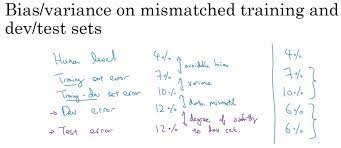
\includegraphics[scale=0.8]{./images/bias_variance_mismatched_data.jpg}
\end{center}

\noindent To solve this issue we create a new set called train-dev set as a random subset of the training set (so it has the same distribution with training set, and we don't use this part of training set to train the model) and we get:

\[\text{Avoidable Bias} = \text{Training error} - \text{Human (Bayes) error}\]
\[\text{Variance} = \text{Training-dev error} - \text{Training error}\]
\[\text{Data mismatch} = \text{Dev error} - \text{Training-dev error}\]
\[\text{Degree of Overfitting to Dev set} = \text{Test error} - \text{Dev error}\]

\noindent \textbf{Addressing data mismatch}:

\noindent There aren't completely systematic solutions to this, but there some things you could try.

\begin{itemize}
    \item Carry out manual error analysis to try to understand the difference between training and dev/test sets.
    \item Make training data more similar to dev/test sets, or collect more data similar to dev/test sets.
\end{itemize}

\noindent If your goal is to make the training data more similar to your dev set, one of the techniques you can use is Artificial data synthesis. (Combine some of your training data with some other data and produce some data that similar to the dev/test set distribution.) For example, combine normal audio with car noise to get audio with car noise example, generate cars using 3D graphics.

\bigskip

\noindent Be cautious and bear in mind whether or not you might be accidentally simulating data only from a tiny subset of the space of all possible examples because your NN might overfit these generated data (like particular car noise or a particular design of 3D graphics cars).

\subsection{Transfer learning}

\noindent Apply the knowledge you took in a task A and apply it in another task B. For example, you have trained a cat classifier with a lot of data, you can use part of the trained NN to solve x-ray classification problem.

\bigskip

\noindent To do transfer learning, delete the last layer(s) of NN and it's weights and:

\begin{itemize}
    \item Option 1: if you have a small data set - keep all the other weights as fixed weights. Add new last layer(s) and initialize the weights for the new layer(s), then feed the new data to the NN and learn the new weights.
    \item Option 2: if you have enough data you can keep less fixed weights and retrain the weights for more layers.
\end{itemize}

\noindent Training on task A called pre-training and Option 1 and 2 are called fine-tuning.

\bigskip

\noindent When transfer learning make sense:

\begin{itemize}
    \item Task A and B have the same input X (e.g. image, audio).
    \item You have a lot of data for the task A you are transferring from and relatively less data for the task B your transferring to.
    \item Low level features from task A could be helpful for learning task B.
\end{itemize}

\subsection{Multi-task learning}

\noindent In multi-task learning, you try to have one neural network do several things at the same time.

\bigskip

\noindent For example, build an object recognition system that detects pedestrians, cars, stop signs, and traffic lights (image has multiple labels). Then Y shape will be \((4,m)\) because we have 4 classes and each one is a binary one.

\bigskip

\noindent Multi-task learning makes sense:

\begin{itemize}
    \item Training on a set of tasks that could benefit from having shared lower-level features.
    \item Usually, amount of data you have for each task is quite similar.
    \item Can train a big enough network to do well on all the tasks.
\end{itemize}

\noindent If you can train a big enough NN, the performance of the multi-task learning compared to splitting the tasks is better. Today transfer learning is used more often than multi-task learning.

\subsection{End-to-end deep learning}

\noindent Some systems break a task into multiple steps, and build a NN for each step. An end-to-end deep learning system implements all these steps with a single NN.

\bigskip

\noindent For example:

\begin{itemize}
    \item Face recognition system. In practice, the best approach is the multi-steps approach for now. It uses one NN for face detection, and another NN which takes two faces as inputs, then outputs if the two faces are the same person or not.
\[\text{Image} --> \text{Face detection} --> \text{Face recognition}\]
\[\text{Image} ------------> \text{Face recognition}\]
    \item Machine translation system. Here end-to-end deep leaning system works better because we have enough data to train the NN.
\[\text{English} --> \text{Text analysis} --> \dots --> \text{French}\]
\[\text{English} ----------------> \text{French}\]
\end{itemize}

\noindent To build the end-to-end deep learning system that works well, we need a big dataset (more data than in non end-to-end system). If we have a small dataset, the multi-steps approach could work better.

\bigskip

\noindent \textbf{Whether to use end-to-end deep learning}:

\noindent Key question: Do you have sufficient data to learn a function of the complexity needed to map X to Y? When applying supervised learning you should carefully choose what types of X to Y mappings you want to learn depending on what task you can get data for.

\bigskip

\noindent Pros of end-to-end deep learning:

\begin{itemize}
    \item By having a pure deep learning approach, your NN learning input from X to Y may be more able to capture whatever statistics are in the data, rather than being forced to reflect human preconceptions.
    \item Less hand-designing of components needed.
\end{itemize}

\noindent Cons of end-to-end deep learning:

\begin{itemize}
    \item May need a large amount of data.
    \item Excludes potentially useful hand-design components (it helps more on the smaller dataset).
\end{itemize}

\noindent Multi-steps approach could be better if a complex system can be divided into multiple tasks and they have a good mapping from data to tasks (autonomous driving), and you are able to build ML/DL models for individual components.

\section{Convolutional Neural Networks}

\subsection{Computer Vision and Convolution}

\noindent Computer vision is one of the applications that are rapidly active thanks to deep learning. Some of the applications of computer vision using deep learning includes self driving cars, face recognition, new types of art...

\bigskip

\noindent Examples of computer vision problems:

\begin{itemize}
    \item Image classification.
    \item Object detection: detect object and localize them.
    \item Neural style transfer: changes the style of an image using another image.
\end{itemize}

\noindent One of the challenges of computer vision problem that images can be so large and we want a fast and accurate algorithm to work with that. For example, a \(1000 \times 1000 \times 3\) image will represent 3 million feature/input to the full connected neural network. If the first hidden layer contains 1000 nodes, then we will have to learn weights of the shape [1000, 3 million] which is 3 billion parameter only in the first layer and that's so computationally expensive! One of the solutions is using convolution layers instead of the fully connected layers.

\bigskip

\noindent \textbf{Edge Detection Examples}

\noindent The convolution operation is one of the fundamentals blocks of a CNN. One of the examples about convolution is the image edge detection operation. Early layers of CNN might detect edges then the middle layers will detect parts of objects and the later layers will put the these parts together to produce an output.

\bigskip

\noindent In an image we can detect vertical edges, horizontal edges, or full edges. Here is an example of convolution operation to detect vertical edges:

\begin{center}
\includegraphics[scale=0.3]{./images/edge_detection.png}
\end{center}

\noindent We slide the \(3 \times 3\) filter(kernel) matrix through the image matrix, each time take 1 step, then get the dot product of the matched matrix and the filter matrix, and the output will be a \(4 \times 4\) matrix.

\bigskip

\noindent In TensorFlow the convolution operation is tf.nn.conv2d. In Keras it is Conv2d.

\bigskip

\noindent Notice that in math textbooks the convolution operation needs to flip the filter before getting the dot product. The "convolution" operation in deep learning field is called cross-correlation operation in mathematics field.

\bigskip

\noindent The vertical edge detection filter will find the \(3 \times 3\) places in an image where it is bright on the left and dark on the right (or in reverse). If we apply this filter to a white region followed by a dark region, it should find the edge in between the two colors as a positive value. But if we apply the same filter to a dark region followed by a white region it will give us a negative value. To solve this we can use the abs function to make it positive.

\bigskip

\noindent \textbf{Vertical edge detection matrix}:

\[
\begin{bmatrix}
1 & 0 & -1\\
1 & 0 & -1\\
1 & 0 & -1
\end{bmatrix}
\]

\noindent \textbf{Horizontal edge detection matrix}:

\[
\begin{bmatrix}
1 & 1 & 1\\
0 & 0 & 0\\
-1 & -1 & -1
\end{bmatrix}
\]

\noindent There are a lot of ways we can put number inside the horizontal or vertical edge detections. For example, the vertical Sobel filter (The idea is taking care of the middle row):

\[
\begin{bmatrix}
1 & 0 & -1\\
2 & 0 & -2\\
1 & 0 & -1
\end{bmatrix}
\]

\noindent Scharr filter (The idea is taking great care of the middle row):

\[
\begin{bmatrix}
3 & 0 & -3\\
10 & 0 & -10\\
3 & 0 & -3
\end{bmatrix}
\]

\noindent To implement convolution in a NN, instead of manually choosing the filter matrix, we can use a matrix of weights that can be learned in the training process, and use the data to learn the right filter matrix for the model. This approach is much more robust than manually choosing the filter.

\[
\begin{bmatrix}
w_{1} & w_{2} & w_{3}\\
w_{4} & w_{5} & w_{6}\\
w_{7} & w_{8} & w_{9}
\end{bmatrix}
\]

\noindent \textbf{Padding}:

\noindent In the last section we saw that a 6x6 matrix convolved with 3x3 filter/kernel gives us a 4x4 matrix. Also we noticed that the pixels in the center of image are used multiple times in the convolution, but the ones at the edge of the image are used less.

\begin{center}
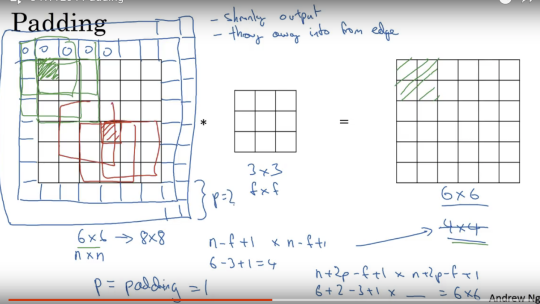
\includegraphics[scale=0.4]{./images/padding.png}
\end{center}

\noindent So the problems with convolutions are:

\begin{itemize}
    \item We want to apply convolution operation multiple times, but if the image shrinks every time we will lose a lot of data in this process.
    \item The edge pixels are used less than central pixels in an image.
\end{itemize}

\noindent To solve these problems we need to use padding. Assume the input image is of shape \(n \times n\), the filter is of shape \(f \times f\), and we add \(p\) padding pixels (of value 0) to the input image. Then the output matrix will be of shape:

\[(n + 2p - f + 1) \times (n + 2p - f + 1)\]

\noindent Choice of padding:

\begin{itemize}
    \item Valid Convolution: \(p = 0\)
    \item Same Convolution: Pad so the output size is the same as input size, using \(p = \frac{f - 1}{2}\). This works when \(f\) is odd, and \(f\) is usually odd in a filter because it's nice to have a central pixel.
\end{itemize}

\noindent \textbf{Strided convolution}:

\noindent When deal with large images, instead of moving 1 step each time, we can move the filter matrix \(s\) steps each time when sliding through the image. Notice that the sliding doesn't happen when there is not enough room to do that. Then the output matrix will be:

\[floor(\frac{n + 2p - f}{s}  + 1) \times floor(\frac{n + 2p - f}{s} + 1)\]

\noindent \textbf{Convolutions Over Volumes}

\noindent We can convolve an image of shape \((height, width, number \ of \ channels)\) (like RGB images) with stacked filters of shape \((height, width, same \ number \ of \ channels)\). To get the convolution of all the channels, we get the the convolution of each channel first and add them together.

\bigskip

\noindent The advantage of using multiple stacked filters is that it helps to detect multiple features in the image.

\begin{center}
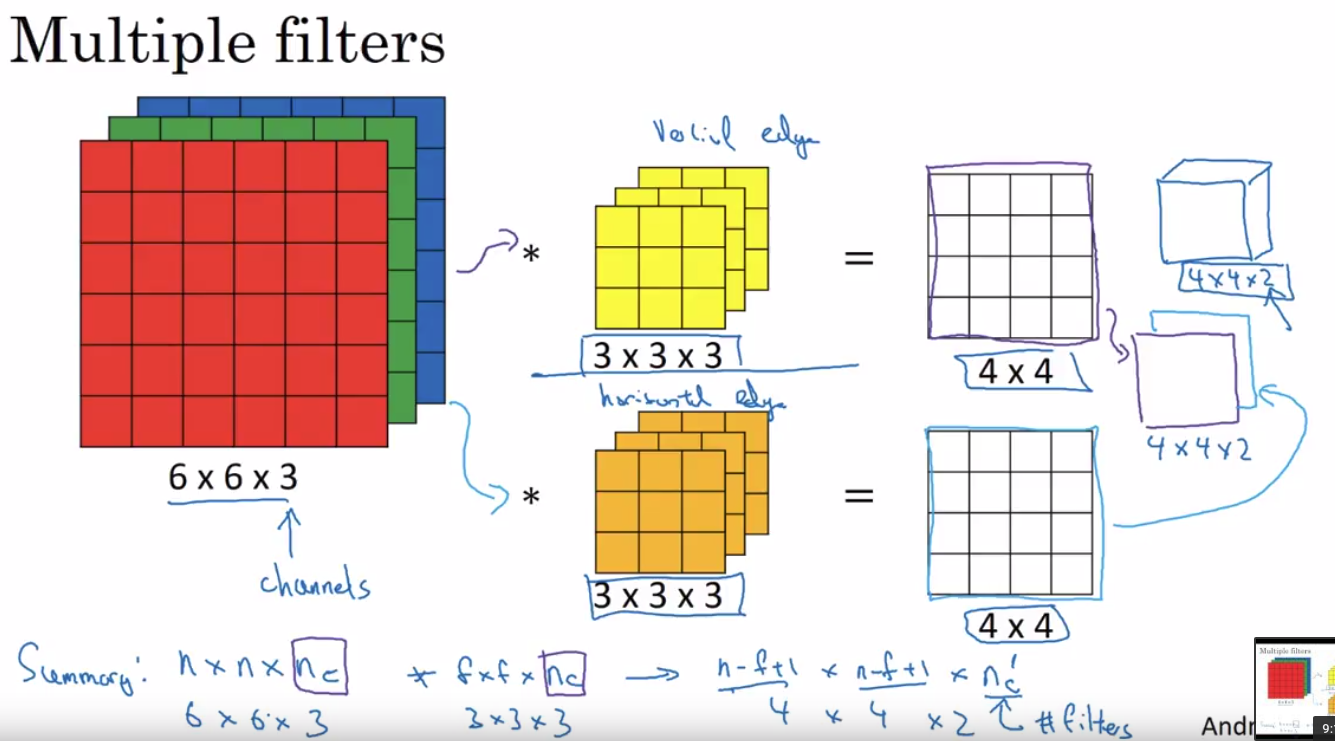
\includegraphics[scale=0.2]{./images/convolutions_over_volumes.png}
\end{center}

\noindent Assume the image is of shape \(n \times n \times n_{c}\), with \(n_{c}^{'}\) stacked filters of shape \(f \times f \times n_{c}\), the output would be of shape \((n - f + 1) \times (n - f + 1) \times n_{c}^{'}\).

\bigskip

\noindent \textbf{One Layer of a Convolutional Net}

\begin{center}
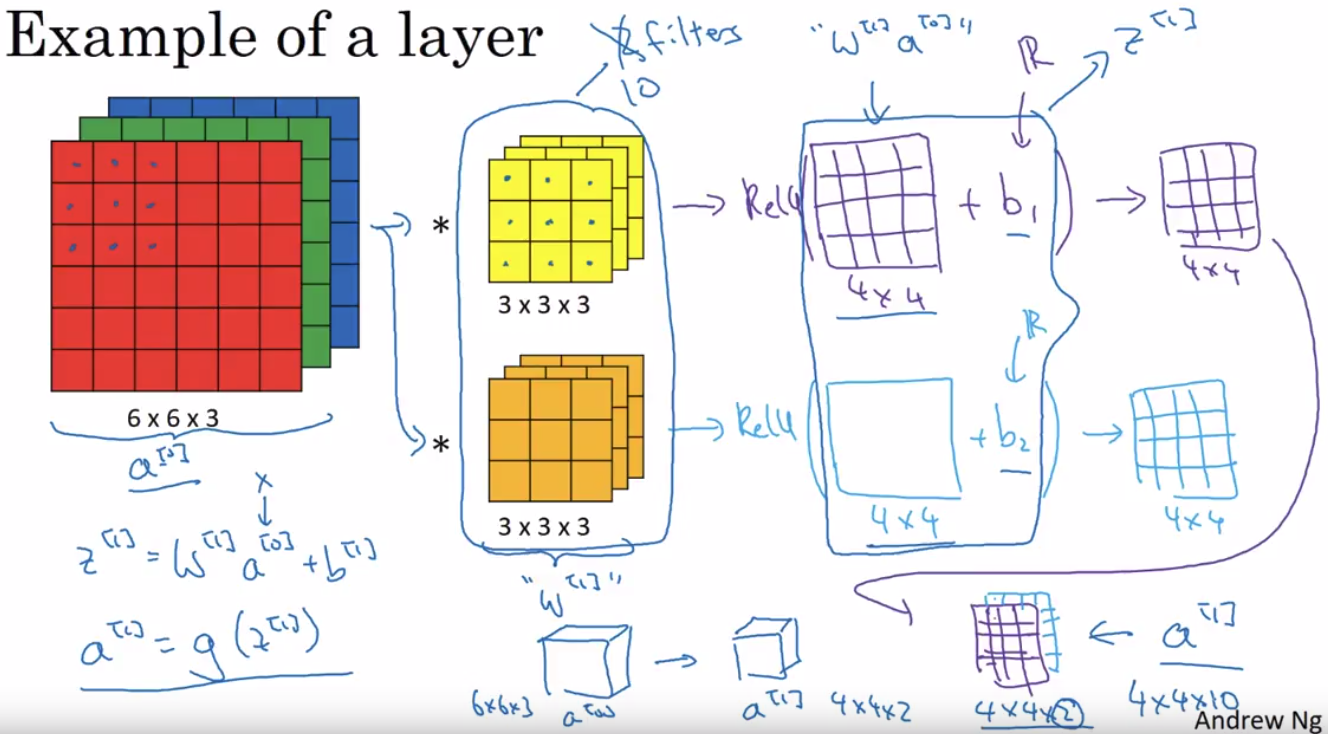
\includegraphics[scale=0.2]{./images/one_layer_of_a_convolutional_net.png}
\end{center}

\noindent If layer \(l\) is a convolutional layer,

\[Input: n_{H}^{[l - 1]} \times n_{W}^{[l - 1]} \times n_{c}^{[l - 1]}\]
\[filter \ width/height = f^{[l]}\]
\[filter \ padding = p^{[l]}\]
\[filter \ stride = s^{[l]}\]
\[filter \ channels = n_{c}^{[l - 1]}\]
\[number \ of \ filters = n_{c}^{[l]}\]
\[n_{H}^{[l]} = floor(\frac{n_{H}^{[l - 1]} + 2p^{[l]} - f^{[l]}}{s^{[l]}} + 1)\]
\[n_{W}^{[l]} = floor(\frac{n_{W}^{[l - 1]} + 2p^{[l]} - f^{[l]}}{s^{[l]}} + 1)\]
\[Output \ a^{[l]}: n_{H}^{[l]} \times n_{W}^{[l]} \times n_{c}^{[l]}\]

\noindent We can find that:

\[Each \ filter \ is \ of \ shape: f^{[l]} \times f^{[l]} \times n_{c}^{[l - 1]}\]
\[Weights \ is \ of \ shape: f^{[l]} \times f^{[l]} \times n_{c}^{[l - 1]} \times n_{c}^{[l]}\]
\[Bias \ is \ of \ shape: n_{c}^{[l]}\]
\[A^{[l]} \ is \ of \ shape: m \times n_{H}^{[l]} \times n_{W}^{[l]} \times n_{c}^{[l]}\]

\noindent \textbf{A simple convolution network example}:

\noindent Here is a simple CNN example:

\begin{center}
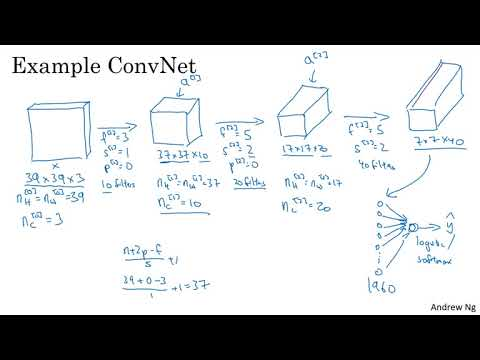
\includegraphics[scale=0.6]{./images/simple_cnn_example.jpg}
\end{center}

\noindent The image goes through 3 convolutional layers, then the output is flattened into a vector so that it can be fed into a logistic regression (or softmax) unit, to be able to classify the image.

\bigskip

\noindent Notice that for the outputs of the convolutional layers, when it goes deeper it's size is shrinking, while it's number of channels is increasing. You can find this trend in many other CNNs.

\bigskip

\noindent Types of layer in a convolutional network:

\begin{itemize}
    \item Convolution Layer.
    \item Pooling Layer.
    \item Fully Connected Layer.
\end{itemize}

\printindex

\end{document}